\chapter{Analysis of Possible Blockchain Technologies for INTERLACE}
\label{ch:dlt}

\vspace{-1cm}
\begin{center}
Paolo Dini and Giuseppe Littera
\end{center}

\section{Introduction}
As stated in the INTERLACE proposal, we are not interested in relying on Bitcoin, due its very low performance efficiency ($< 10$ transactions per second, or $[Tx/s]$) and the wastefully high energy requirements of the Proof of Work (PoW) consensus protocol. Bitcoin, however, remains a useful reference point for many blockchain properties and parameters. It is therefore assumed that the reader is already familiar with the basic concepts of the Bitcoin blockchain, which are extremely well-explained in the excellent book by Antonopoulos \cite{Antonopoulos2015}.

In the next section we present a few important concepts around which design trade-offs, and in our case selection trade-offs, have been made to arrive at the architecture that we feel is most suitable for INTERLACE and for the Sardex circuit. A few more specific details are then presented that concern a small subset of possible Distributed Ledger Technologies (DLTs) in common use, which are summarised at the end of the chapter in a summary table. Thus, the analysis in this chapter forms the basis for the architectural design decisions described in Chapter \ref{ch:hl}.

\section{Basic Concepts}
\subsection{The Blockchain as a Distributed Applications Platform}
The most important innovation implicit in the Bitcoin blockchain is not the creation ``out of thin air'' of a new currency, or the substitution of a central authority for validating a ledger of transactions in this new independent currency with a distributed architecture based on a consensus protocol. These two innovations were the main motivation for creating Bitcoin, but as has been noted countless times the potentially more impactful innovation is the blockchain itself. Figure \ref{fig:dapps} proposes a reason why by highlighting the role of the second-generation blockchains such as Ethereum as a distributed, permanent, and immutable memory in enabling a new type of distributed application. The fact that this memory substrate is shared among completely unrelated applications and user groups is interesting from the point of view of the sharing economy, which could be regarded as a third innovation, but the (fourth) innovation that opens up a new space for computer science and software engineering is the fact that the memory is \emph{distributed}, \emph{permanent}, and \emph{immutable}.

As shown in Figure \ref{fig:dapps}, whereas Bitcoin allows only for the simplest kinds of interactions between users and the permanent, distributed, and immutable memory, second-generation blockchains have introduced what looks like a familiar stack: user interface, code, persistence layer. However, the persistence layer is writable only once. A permanent and immutable \emph{shared} history will remain ``on the \emph{shared} record'' forever -- or at least as long as the human species lasts. Clearly, this is a very special type of application that has never been possible before. If, as Edward De Bono said long ago, memory is the basic mechanism of intelligence \cite{DeBono1969}, this kind of persistence layer could be the start of a collective intelligence with properties and capabilities that are impossible to predict today. For the moment, therefore, we focus on the most obvious use case, a financial information system -- i.e.\ as the blockchain as the ``mind'' of the real economy. In particular, we wish to define the most appropriate properties of the financial information system and transaction engine for the Sardex circuit.

\begin{figure}[h]
\centering
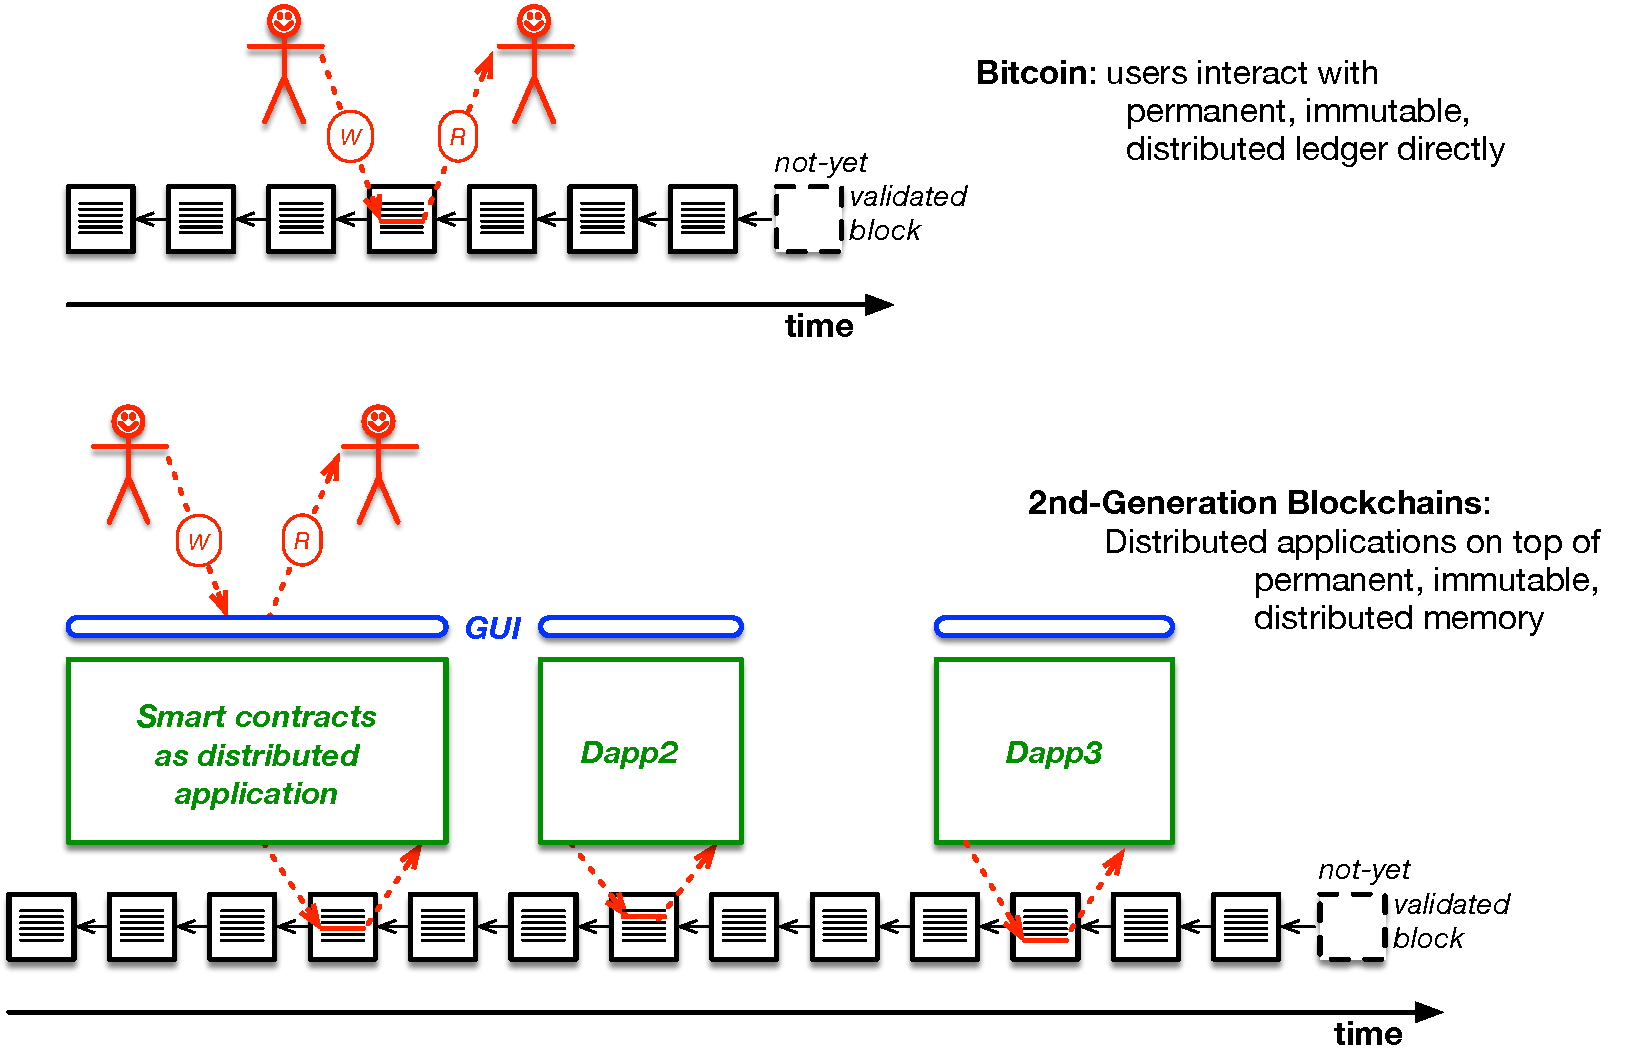
\includegraphics[width=17 cm]{Figures/dapps}
\caption{\bf \small Second-generation blockchains enable a peculiar type of distributed application}
\label{fig:dapps}
\end{figure}

As explained in the Corda technical white paper (\cite{Hearn2016}: 30), the need for organising the transactions into blocks is a consequence of the fact that the rate at which transactions are performed is greater than the rate at which they can be validated by all the peers of a large distributed system with network latencies. The block structure permits the validation of a set of transactions at a time. Since Corda is a permissioned distributed database, it does not need to achieve global consensus and therefore does not need to employ blocks.

\subsection{Deterministic Execution}
As discussed in the Hyperledger technical white paper \cite{AndroulakiEtAl2018}, distributed systems have relied on the state machine replication (SMR) paradigm \cite{Schneider1990} for a few decades. The SMR approach is motivated by the need for redundancy in the provision of services to a given client as a strategy to offset possible faults. Each service request from a client is executed in an identical, deterministic, and asynchronous way by a set of servers, which means that the same operations are executed in the same order by each server, even though not necessarily at the same time. By definition, the correct response is whatever the majority of the servers calculates. Therefore, SMR is resistant also to Byzantine faults, which are malicious and not merely technical. More precisely, an SMR system is $t$-resistant as long as no more than $t$ servers are affected by faults (Byzantine or otherwise) for a total set comprising $2t + 1$ servers. Most blockchains have taken SMR as a starting point, where the set of operations in this case is one block of transactions. In particular, most global consensus algorithms are centred around reaching agreement on the ordering of the transactions in a given block -- hence the name `order-execute' for this type of distributed architecture.

For example, in Bitcoin order-execute involves deterministic sequential execution by each peer, after the first peer has ordered a block, solved the PoW puzzle, and broadcast the block by gossip. The validation of the new block is achieved once every peer has completed and validated the execution. In a public blockchain such as Ethereum a denial-of-service (DoS) attack could be mounted by embedding an infinite loop in the smart contract of one of the transactions. Since it is not possible to determine in general whether or not an algorithm completes (`halting problem'), such a loop could go undetected, leading to a block that cannot be validated and stopping the ability of the blockchain to support future transactions. Ethereum solves this problem by using ``gas'' which, once converted in the cryptocurrency of that blockchain (ether), results in a charge for the execution of transactions.

The low efficiency of sequential execution can be improved upon with parallel execution of unrelated transactions. However, detecting the possible interdependencies is not trivial. Stellar and Holochain seem to have been able to do that.

\subsection{Non-Deterministic Execution}
Non-deterministic execution of smart contracts can lead to forks in the blockchain and is therefore avoided when possible. This can be achieved by means of smart contract languages that are not Turing-complete: they should be expressive enough for the purposes of the blockchain they serve (like Solidity for Ethereum) but not so general as to render complete avoidance of non-determinism impossible. For example, Androulaki et al.\ \cite{AndroulakiEtAl2018} mention a map iterator in Go that is a deterministic operation at the level of the command but hides a non-deterministic implementation in the Go language itself.

\subsection{Confidentiality}
Performing chaincode on all peers may expose details that some peer would rather be kept private. This issue is particularly important in B2B contexts. One possible solution is to replicate the end-state of the calculation (passive replication) rather than the whole calculation (active replication) \cite{AndroulakiEtAl2018}.

\subsection{Native Currency}
The Bitcoin blockchain provides the simplest example of what a native currency is and how it is created. This is done by a miner by writing a transaction to self of (currently) 12.5 BTC at the beginning of the block he/she will then try to validate by finding the nonce that satisfies the puzzle requirement (i.e.\ the hash of the miner's current block with the winning nonce) for the current block. If the miner wins the current PoW puzzle the 12.5 BTC to self will become ``real'' and will be credited to her private key. Many blockchains, like Hyperledger, do not have a native currency. This is what INTERLACE needs because in mutual credit the important concept is not whether or not an \emph{asset} is present but what value someone's credit \emph{balance} has -- a value that can be negative as well as positive.


\subsection{Latency vs.\ Performance in Consensus}
As shown in Figure \ref{fig:consensus_tradeoffs}, the consensus objective can be cast as a trade-off between network latency vs.\ blockchain performance expressed in transactions per second [$Tx/s$] (\cite{vukolic2015}, cited in \cite{AndroulakiEtAl2018})




\begin{figure}[h]
\centering
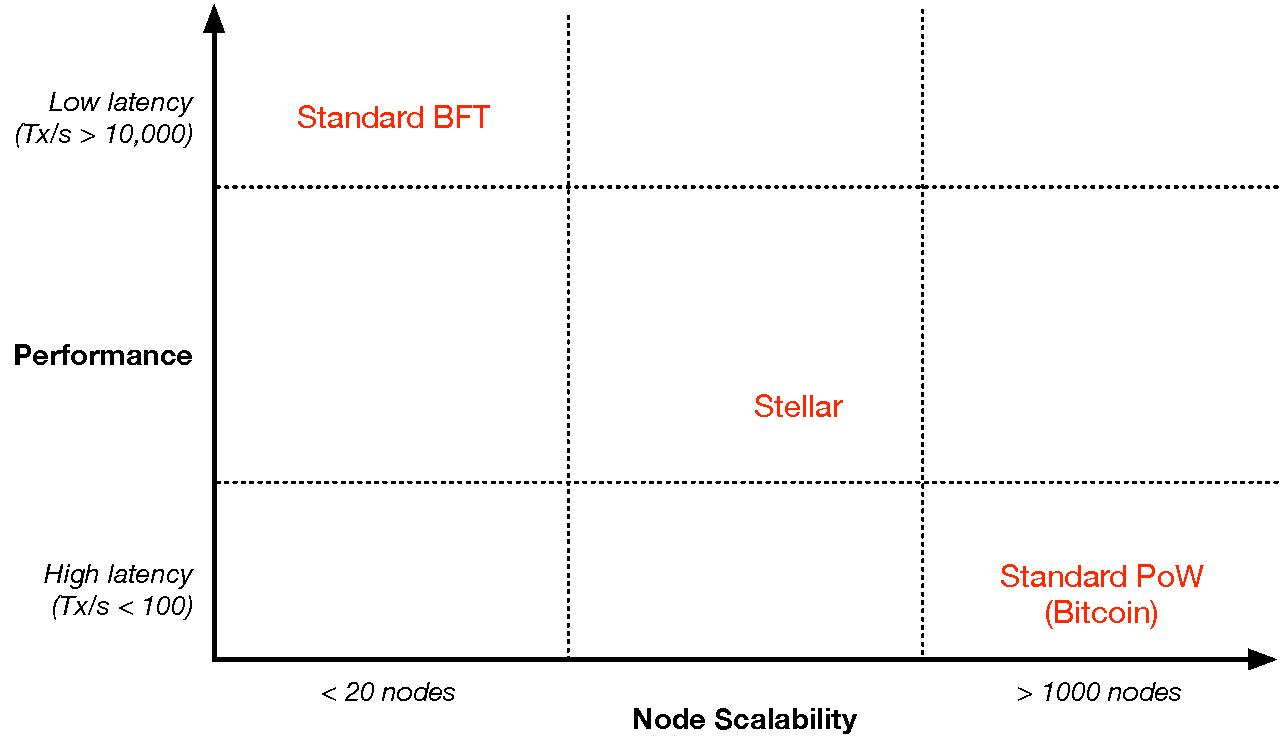
\includegraphics[width=14 cm]{Figures/consensus_tradeoffs}
\caption{\bf \small Network latency-node scalability trade-offs, after \cite{vukolic2015}}
\label{fig:consensus_tradeoffs}
\end{figure}









\section{Brief Summary of Some DLT Technologies}

The INTERLACE team has looked at a number of blockchain technologies:
\begin{packed_item1}
\item Corda
\item Holochain
\item Stellar
\item Quorum (permissioned Ethereum)
\item Hyperledger Fabric
\end{packed_item1}
In this chapter we analyse and discuss them briefly in turn, emphasising the algorithmic, architectural,  mathematical, or financial aspects that are most pertinent to INTERLACE. The frameworks that have made it into this short list are all interesting for one reason or another, and at different points each of them was seriously taken into consideration for adoption. Stellar has an interesting mathematical foundation which is therefore studied and discussed in some detail since mathematical understanding can be transferred to other frameworks. The one that comes closest to the requirements of the Sardex mutual credit system is Hyperledger. Therefore, after presenting and discussing the others Hyperledger will be analysed and presented in more detail.


\subsection{Corda}
Corda \cite{Hearn2016} is a permissioned distributed database for banking networks. It does not use a blockchain



\subsection{Holochain}
Agent-centric
\cite{HarrisBrownEtAl2018}








\subsection{Stellar}


\subsection{Quorum}

\footnote{\url{https://github.com/jpmorganchase/quorum-docs/blob/master/Quorum_Architecture_20171016.pdf}}



\subsection{Hyperledger}
The main points of interest of Hyperledger Fabric are \cite{AndroulakiEtAl2018}:

\begin{quote}
\begin{packed_item1}
\item It supports modular consensus protocols, which allows the system to be tailored to particular use cases and trust models.
\item Fabric is the first blockchain system that runs distributed applications written in standard, general-purpose programming languages, without systemic dependency on a native cryptocurrency. This stands in sharp contrast to existing blockchain platforms that require �smart-contracts� to be written in domain-specific languages or rely on a cryptocurrency.
\item Fabric realizes the permissioned model using a portable notion of membership, which may be integrated with industry-standard identity management.
\item Fabric achieves end-to-end throughput of more than 3500 transactions per second in certain popular deployment configurations, with sub-second latency, scaling well to over 100 peers.
\end{packed_item1}
\end{quote}



Hyperledger Indy-Plenum Byzantine Fault Tolerance (PBFT).\footnote{\url{https://github.com/hyperledger/indy-plenum/wiki}} PBFT is based on RBFT: Redundant Byzantine Fault Tolerance
\cite{Aublinetal2013}.






%&\hspace{0.5cm}ASM/ASIM framework \\





\begin{sidewaystable}
\small
\begin{centering}
{\begin{tabular}{| l | c | c | c | c | c | c | c | c | c | c |}
\hline
				& 				& \textbf{Read}			& \textbf{Write}		& \textbf{} 
				& \textbf{Smart}		& \textbf{Smart}			&\textbf{Consensus}
				& \textbf{Backup} 	& \textbf{}				&\textbf{Monetary} \\
\textbf{DLT}		&\textbf{Focus}  	& \textbf{Access} 		& \textbf{Access}	& \textbf{Data/Agent} 
				& \textbf{Contracts} 	& \textbf{Contract}		&\textbf{Model} 
				& \textbf{System} 	& \textbf{Interfaces}		&\textbf{Model} \\
				& 				& \textbf{} 				& \textbf{} 			& \textbf{} 
				& \textbf{} 			& \textbf{Language(s)}	&\textbf{} 
				& \textbf{} 			& \textbf{}				&\textbf{} \\
\hline
\hline
\textbf{Ethereum}	&General-purpose		&Public		&Permissionless	&Data-centric	&Yes		&Solidity	
				&Global, PoS 			&?			&?				&Assets \\
				&platform 				&			&				&			&		&on EVM	
				& 					&			&				& \\
\hline
\textbf{Holochain}	&Fog 				&Public		&Permissionless	&Agent-centric	&?		&?
				&Local 				&?			&?				&Mutual Credit\\
\hline
\textbf{Stellar}		& 					&Public		&Permissionless	&Data-centric	&?		&
				&FBAS 				&?			&?				&Assets\\
\hline
\textbf{Corda} 		&Business agreements	&Private		&Permissioned		&Data-centric	&?		&Bytecode
				&Local state			&Relational DB	&SQL			&Assets\\
		 		&between financial inst.	&			&				&			&		&subset on JVM
				&(Notaries)			&			&FPML			&\\
\hline
\textbf{Quorum} 	&Public and  			&Private		&Permissioned		&Data-centric	&?		&
				&BFT 				&?			&?				&Assets\\
			 	&banking sectors		&			&				&			&		&
				& 					&			&				&\\
\hline
\textbf{Hyperledger}	&Enterprise, B2B		&Private		&Permissioned		&Data-centric	&Yes		&JS, Go
				&Centralised 			&Key-value	&?				&Adaptable to\\
 				& \& supply chain		&			&				&			&		&
				& 					&store DB		&				&Mutual Credit\\
\hline
\end{tabular}}

\vspace{1cm}

{\begin{tabular}{| l | c | c | c | c | c | c | c | c | c | c |}
\hline
				& \textbf{}  			& \textbf{}  			& \textbf{Transaction} 	&
				& \textbf{Regulatory/} 	& \textbf{Explicit links}	&\textbf{Business}
				& \textbf{Computational} 	& \textbf{Turing}		&\textbf{Contract} \\
\textbf{DLT}		& \textbf{Blockchain} 	& \textbf{Immutable} 		& \textbf{Validation} 		& \textbf{Architecture} 
				& \textbf{Supervisory} 	& \textbf{of SCs to}		&\textbf{Flow} 
				& \textbf{Model} 		& \textbf{Completeness}	&\textbf{Object} \\
				& \textbf{} 				& \textbf{} 				& \textbf{} 				&
				& \textbf{nodes} 		& \textbf{legal prose}		&\textbf{} 
				& \textbf{} 				& \textbf{}				&\textbf{} \\
\hline
\hline
\textbf{Ethereum}	&Yes			&Yes		&				&Order-Execute	&
				&			&		&Virtual Computer	&No				&Stateful \\
\hline
\textbf{Holochain}	&Individual	&?		&Local to the parties	&				&
				&			& 		&				&				& \\
				&chains		&		&				&				&
				&			& 		&				&				& \\
\hline
\textbf{Stellar}		&			&?		&				&				&?
				&			& 		&?				&?				&\\
\hline
\textbf{Corda} 		&No			&Yes		&Local to the parties	&				&Yes
				&			&Yes		&UTXO			&Yes				&Stateless\\
\hline
\textbf{Quorum} 	&Yes			&?		&				&Order-Execute	&?
				&			& 		&?				&?				&\\
\hline
\textbf{Hyperledger}	&Yes			&Yes		&				&Execute-Order	&
				&			& 		&?				&?				& \\
 				&			&		&				&Validate			&
				&			& 		&				&				& \\
\hline
\end{tabular}}


\vspace{1cm}

{\begin{tabular}{| l | c | c | c | c | c | c | c | c | c | c |}
\hline
				& \textbf{Inter-Node}		& \textbf{}  			& \textbf{} 	&
				& \textbf{} 				& \textbf{}				&\textbf{}
				& \textbf{} 				& \textbf{}				&\textbf{} \\
\textbf{DLT}		& \textbf{Communication} 	& \textbf{} 				& \textbf{} 		& \textbf{} 
				& \textbf{} 				& \textbf{}				&\textbf{} 
				& \textbf{} 				& \textbf{}				&\textbf{} \\
				& \textbf{} 				& \textbf{} 				& \textbf{} 				&
				& \textbf{} 				& \textbf{ }				&\textbf{} 
				& \textbf{} 				& \textbf{}				&\textbf{} \\
\hline
\hline
\textbf{Ethereum}	&Global			&		&				&	&
				&			&		&	&				& \\
\hline
\textbf{Holochain}	&Local		&?		&	&				&
				&			& 		&				&				& \\
				&			&		&				&				&
				&			& 		&				&				& \\
\hline
\textbf{Stellar}		&			&?		&				&				&?
				&			& 		&?				&?				&\\
\hline
\textbf{Corda} 		&Flows			&		&&				&
				&			&		&			&				&\\
\hline
\textbf{Quorum} 	&			&?		&				&	&?
				&			& 		&?				&?				&\\
\hline
\textbf{Hyperledger}	&			&		&				&	&
				&			& 		&?				&?				& \\
 				&			&		&				&			&
				&			& 		&				&				& \\
\hline
\end{tabular}}


\caption{\bf \small Summary table comparing the main properties of different types of blockchain}
\label{blockchain_type}
\end{centering}
\end{sidewaystable}





